\documentclass[11pt,a4paper,oneside]{article}
\usepackage[dutch]{babel}
\usepackage{amsmath}
\usepackage{graphicx}
\usepackage{tikz}
\usepackage{fancyhdr}
\usepackage{dsfont}
\usepackage{parskip}
\usepackage{epstopdf}
\usepackage{listings}
\usepackage{color}
\definecolor{lichtgrijs}{gray}{0.95}
\usepackage{cite}
\usepackage[nottoc]{tocbibind}
\usepackage[T1]{fontenc}
\usepackage[light,math]{iwona}
\usepackage{pgfplots}
\pgfplotsset{compat=newest}
\usepackage{subfig}
\usepackage{textcomp}
\usetikzlibrary{arrows,automata}
\usepackage{float}
\usepackage{longtable}
\usepackage{titling,enumitem}
\usepackage{a4wide}
\usepackage{amssymb}
\usepackage{rotating}
\usepackage{listings}
\usepackage[top=1.1in, bottom=1.2in, left=1.1in, right=1.1in]{geometry}
\usepackage{array}
\usepackage{titling}
\usepackage{blindtext}
\usepackage{chngpage}
\usepackage{calc}
\definecolor{lightgray}{gray}{0.8}
\newcolumntype{L}{>{\raggedleft}p{0.50\textwidth}}
\newcolumntype{R}{p{0.8\textwidth}}
\newcommand\VRule{\color{lightgray}\vrule width 0.5pt}
\usepackage{color, colortbl}
\definecolor{Gray}{gray}{0.9}
\definecolor{dkgreen}{rgb}{0,0.6,0}
\definecolor{gray}{rgb}{0.5,0.5,0.5}
\definecolor{mauve}{rgb}{0.58,0,0.82}
\definecolor{ugentblue}{rgb}{0.05,0.18,0.37}
\usepackage{import}
\usepackage[T1]{fontenc}
\begin{document}

\newgeometry{top=0.8cm, right=1.70cm, left=1.7cm}
\begin{titlepage}

\thispagestyle{fancy}
\fancyhf{}
\fancyfoot[L]{}
\begin{figure}[!ht]
  \begin{adjustwidth}{-\oddsidemargin-1in}{-\rightmargin}
    \centering
    
\includegraphics[width=\paperwidth]{banner}
  \end{adjustwidth}
\end{figure}
\vspace{-0.2em}
\begin{center}
\vspace{5cm}
\Huge \textbf{Vakoverschrijdend Project: team Edran\\ Rapport episode 1}\\
\vspace{6.0cm}
\large
\begin{tabular}{L! {} R}
& {\LARGE\bf Team Edran} \\
& \\
& {\bf Steven De Blieck} \\
& {\bf Laurens De Graeve} \\
& {\bf Bart Middag} \\
& {\bf Wouter Pinnoo} \\
& {\bf Robin Praet} \\
& {\bf Stijn Seghers} \\
& {\bf Wouter Termont} \\
& {\bf Gilles Vandewiele} \\
\end{tabular}
\end{center}
\end{titlepage}
\restoregeometry
\newpage

\fancyheadoffset[RO,LE]{0in}
\fancypagestyle{plain}{
\fancyhead[L]{Rapport episode 1}
\fancyhead[R]{Team Edran}
\fancyfoot[L]{}
\fancyfoot[R]{\thepage}}

\fancyhead[L]{Rapport episode 1}
\fancyhead[R]{Team Edran}
\fancyfoot[L]{}
\fancyfoot[C]{\thepage}
\pagestyle{fancy}
\tableofcontents
\newpage
\part{Verwachte functionaliteiten}
\begin{itemize}
	\item Ritten reserveren en reservaties goedkeuren/afkeuren
	\item Registeren voor infosessie
	\item Standaard-emails, die ge\"{e}diteerd kunnen worden door een beheerder, versturen door het systeem
\end{itemize}

\part{Actoren van het systeem}
\begin{itemize}

	\item Gewone gebruiker: een geregisteerde persoon die nog geen lid van de VZW is.
	\item Eigenaar: \emph{verantwoordelijke} eigenaar en \emph{gepriviligeerde} eigenaar
	\item Autolener
	\item Beheerder:  is niet verder opgedeeld omdat er in het systeem met machtigingen zal gewerkt worden. Er zijn dus verschillende soorten beheerders, naargelang de machtigingen die ze toegewezen kregen.
	
\end{itemize}

\part{Het reserveren van ritten en goedkeuren/afkeuren van reservaties}

\section{Usecases}

\subsection{Auto + tijdstip bekijken}
\begin{itemize}
\item \textbf{Precondities:} autolener is ingelogd
\item \textbf{Trigger:} autolener bekijkt kalender
\item \textbf{Acties:} \begin{itemize}
\item	autolener zoekt op basis van tijdstip, naam auto, capaciteit auto, geografische standplaats
\item	systeem geeft meest passende mogelijke reservaties eerst terug
\item	autolener kiest auto + tijdstip 
\item 	systeem geeft details reservatie terug (naam auto, tijdstip, capaciteit, standplaats) + de naburige autoleners hun naam, telefoonnummer en emailadres
\end{itemize}
\item \textbf{Postcondities:} auto + tijdstip weergegeven
\end{itemize}


\subsection{Auto reserveren} \label{reserveren}
\begin{itemize}
\item \textbf{Precondities:} autolener is ingelogd, autolener bekijkt auto + tijdstip
\item \textbf{Trigger:} autolener kiest reserveren
\item \textbf{Acties:} \begin{itemize}
\item 	autolener geeft duur aan van de reservatie
\item systeem controleert of auto beschikbaar is voor deze duur
\item systeem slaat reservatie op in DB
\item      systeem laat autolener weten dat reservatie is gelukt
\item      systeem informeert eigenaar van de reservatie zodat deze die kan afhandelen
\end{itemize}
\item \textbf{Postcondities:} reservatie is toestand 'aanvraag'
\end{itemize}


\subsection{Eigenaar keurt reservatie goed}
\begin{itemize}
\item \textbf{Precondities:} eigenaar is ingelogd en bekijkt zijn reservatie-aanvragen \item \textbf{Trigger:} eigenaar kiest bepaalde reservatie
\item \textbf{Acties:} \begin{itemize}
\item	eigenaar kiest goedkeuren
	
\item	systeem slaat reservatie op in DB
\item      systeem laat eigenaar weten dat goedkeuren is gelukt
\item      systeem informeert autolener van de goedkeuring
\end{itemize}
\item \textbf{Postcondities:} reservatie is toestand 'goedgekeurd'
\end{itemize}


\subsection{Eigenaar weigert reservatie}
\begin{itemize}
\item \textbf{Precondities:} eigenaar is ingelogd en bekijkt zijn reservatie-aanvragen \item \textbf{Trigger:} eigenaar kiest bepaalde reservatie
\item \textbf{Acties:} \begin{itemize}
\item	eigenaar kiest weigeren
\item	eigenaar voegt korte reden toe voor weigering
\item	systeem slaat reservatie op in DB
\item      systeem laat eigenaar weten dat weigeren is gelukt
\item      systeem informeert autolener van de weigering
\end{itemize}
\item \textbf{Postcondities:} reservatie is toestand 'geweigerd'
\end{itemize}

\subsection{Autolener annuleert reservatie}
\begin{itemize}
\item \textbf{Precondities:} autolener is ingelogd en bekijkt zijn reservaties \item \textbf{Trigger:} autolener kiest bepaalde reservatie
\item \textbf{Acties:} \begin{itemize}
\item	eigenaar kiest annuleren
\item	systeem slaat reservatie op in DB
\item      systeem laat autolener weten dat annuleren is gelukt
\item      systeem informeert eigenaar van de annulatie
\end{itemize}
\item \textbf{Postcondities:} reservatie is toestand 'geannuleerd'
\end{itemize}

\subsection{Autolener verkort reservatie}
\begin{itemize}
\item \textbf{Precondities:} autolener is ingelogd en bekijkt zijn reservaties \item \textbf{Trigger:} autolener kiest bepaalde reservatie
\item \textbf{Acties:} \begin{itemize}
\item	autolener kiest inkorten
\item	autolener kiest nieuwe duur
\item	systeem controleert of auto beschikbaar is voor deze duur
\item	systeem slaat reservatie op in DB
\item      systeem laat autolener weten dat inkorten is gelukt
\item      systeem informeert eigenaar van de inkorting
\end{itemize}
\item \textbf{Postcondities:} reservatie is ingekort
\end{itemize}

\subsection{Eigenaar reserveert eigen auto}
\begin{itemize}
\item \textbf{Precondities:} eigenaar is ingelogd, eigenaar bekijkt zijn eigen auto
\item \textbf{Trigger:} eigenaar kiest tijdstip
\item \textbf{Acties:} \begin{itemize}
\item	eigenaar kiest reserveren
\item 	eigenaar kiest duur reservatie
\item	systeem controleert of auto beschikbaar is voor deze duur
\item	systeem slaat reservatie op in DB
\item      systeem laat eigenaar weten dat reservatie is gelukt
\end{itemize}
\item \textbf{Postcondities:} reservatie is toestand 'goedgekeurd'
\end{itemize}

\section{Mockups}
\begin{center}

\begin{figure}[H]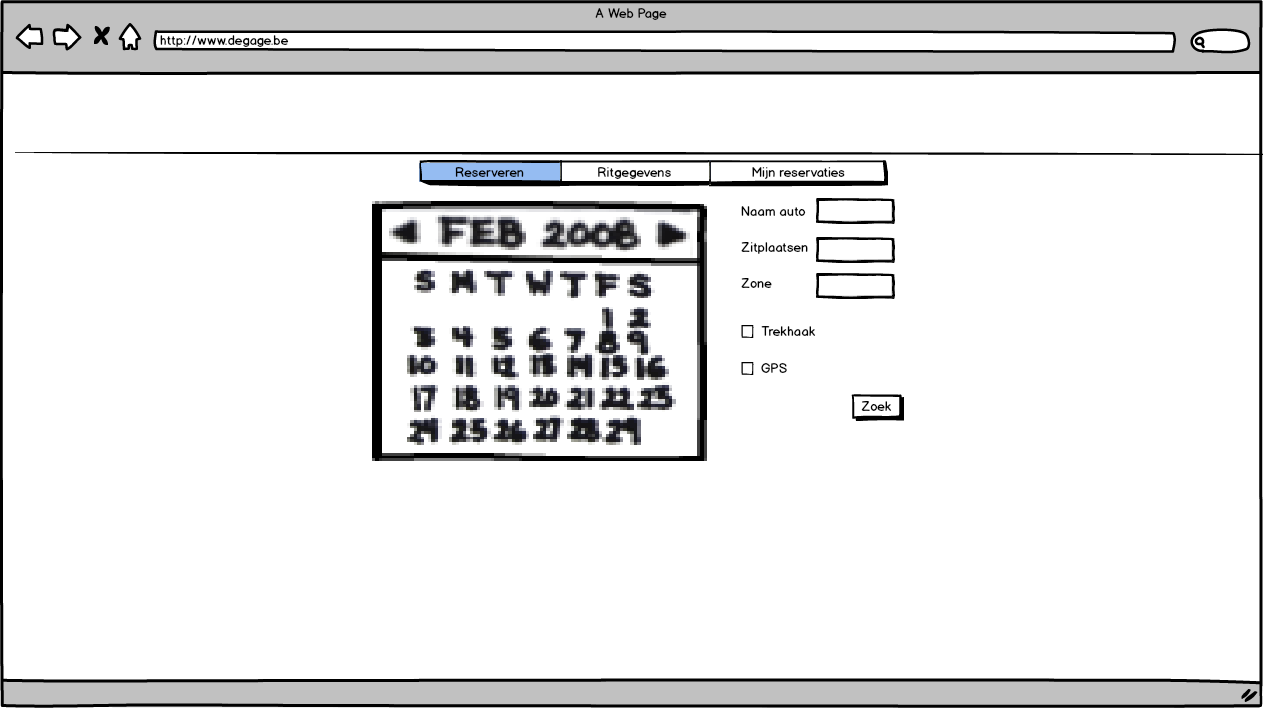
\includegraphics[width=\textwidth]{../../mockups/delen_reserveren.png}\end{figure}

\begin{figure}[H]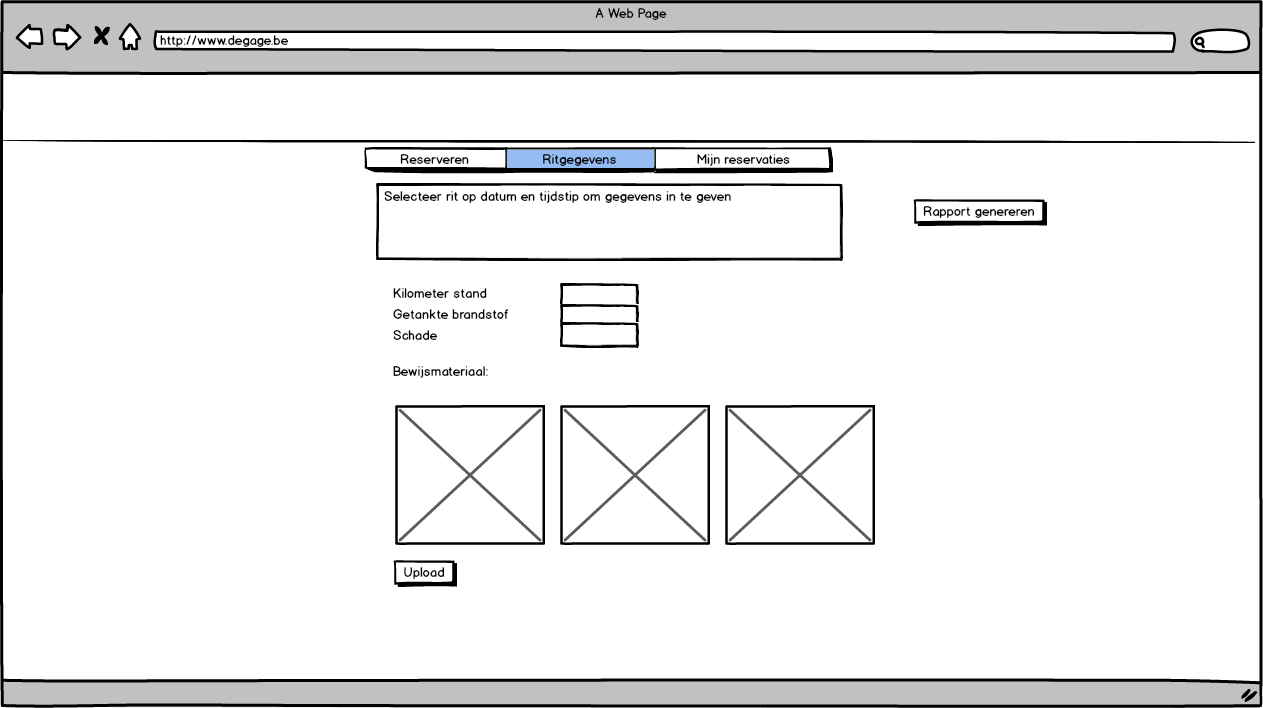
\includegraphics[width=\textwidth]{../../mockups/delen_ritgegevens.png}\end{figure}

\begin{figure}[H]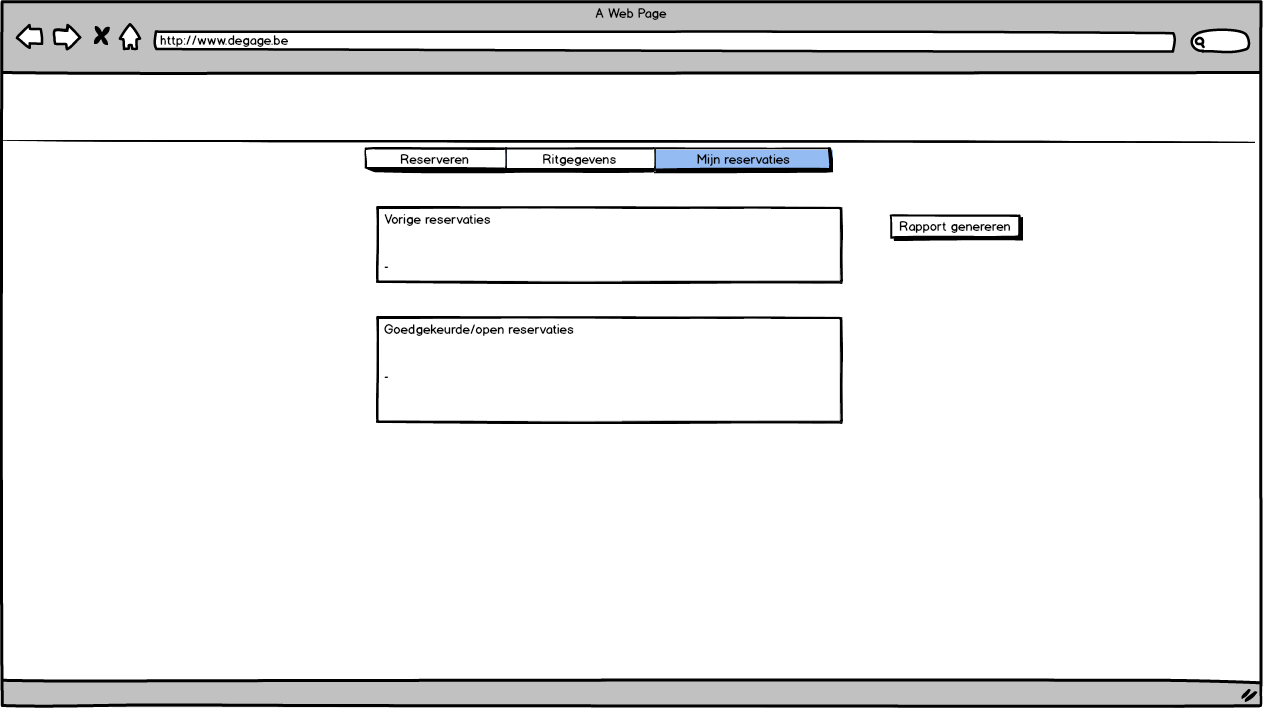
\includegraphics[width=\textwidth]{../../mockups/delen_mijnreservaties.png}\end{figure}

\begin{figure}[H]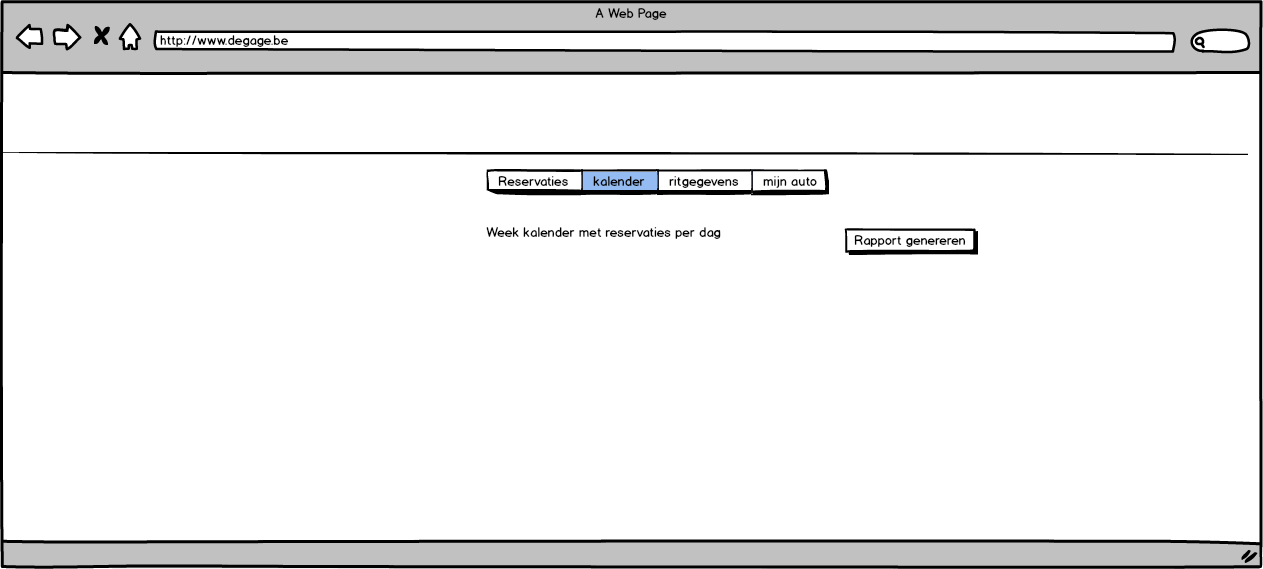
\includegraphics[width=\textwidth]{../../mockups/autobeheer_kalender.png}\end{figure}

\begin{figure}[H]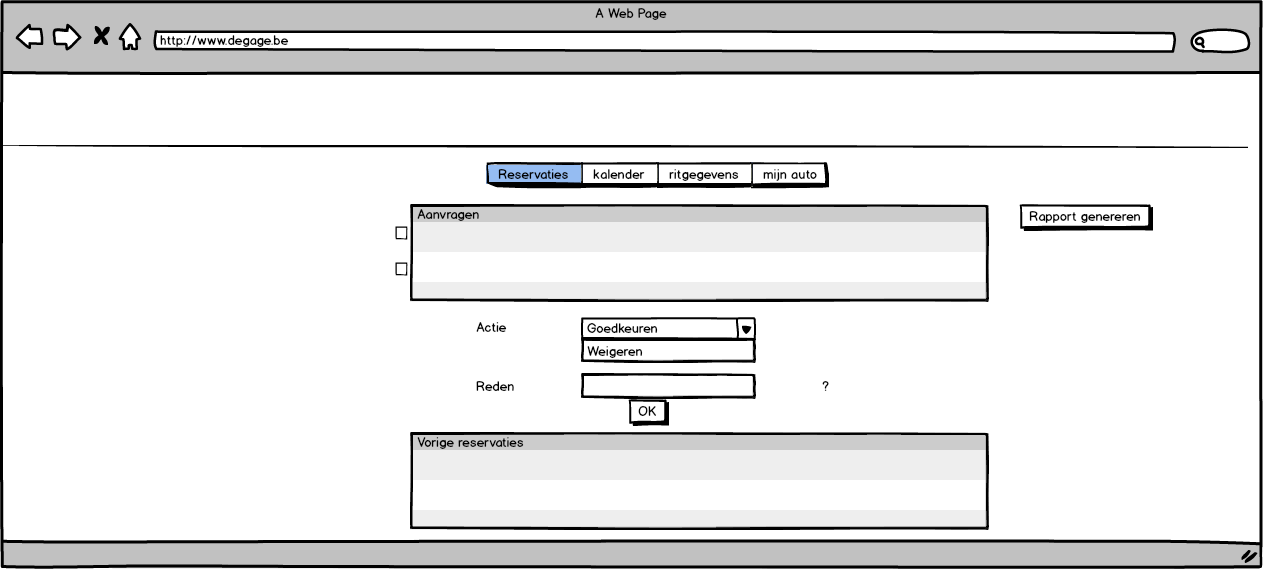
\includegraphics[width=\textwidth]{../../mockups/autobeheer_reservaties.png}\end{figure}

\end{center}

\setcounter{section}{0}
\setcounter{subsection}{0}
\part{Registeren voor infosessie}

\section{Usecases}


\subsection{Inschrijven infosessie}
\begin{itemize}

\item \textbf{Precondities:} gewone gebruiker is ingelogd
\item \textbf{Trigger:} gebruiker kiest een bepaalde infosessie op de kalender of op een aparte pagina voor infosessies 
\item \textbf{Acties:} \begin{itemize}
\item	gebruiker kiest inschrijven
\item	de gebruiker krijgt een bericht van het systeem dat de inschrijving is gelukt
\item	het systeem voegt de gebruiker toe aan een lijst van aanwezigen bij een bepaalde infosessie
\end{itemize}
\item \textbf{Postcondities:} De gebruiker krijgt de toestand \emph{aanwezig/ingeschreven}.
\end{itemize}

\subsection{Uitschrijven infosessie}
\begin{itemize}

\item \textbf{Precondities:} gewone gebruiker is ingelogd
\item \textbf{Trigger:} gebruiker kiest een bepaalde infosessie op de kalender waarvoor hij op aanwezig staat 
\item \textbf{Acties:} \begin{itemize}
\item	gebruiker kiest uitschrijven
\item	de gebruiker krijgt een bericht van het systeem dat de uitschrijving is gelukt
\item	het systeem verwijdert de gebruiker van de lijst van aanwezigen bij een bepaalde infosessie
\end{itemize}
\item \textbf{Postcondities:} De gebruiker krijgt de toestand \emph{afwezig}.
\end{itemize}


\subsection{Infosessie aanmaken}
\begin{itemize}
\item \textbf{Precondities:} beheerder is ingelogd en bekijkt infosessies
\item \textbf{Trigger:} beheerder kiest nieuwe infosessie aanmaken
\item \textbf{Acties:} \begin{itemize}
\item	beheerder geeft datum, tijdstip, locatie en beschrijving nieuwe infosessie in
\item 	systeem slaat dit op in DB
\item	systeem laat weten aan beheerder dat de infosessie in aangemaakt
\end{itemize}
\item \textbf{Postcondities:} infosessie aangemaakt
\end{itemize}

\subsection{Details infosessie bekijken}
\begin{itemize}
\item \textbf{Precondities:} beheerder is ingelogd en bekijkt infosessies
\item \textbf{Trigger:} beheerder kiest bepaalde infosessie
\item \textbf{Acties:} \begin{itemize}
\item	beheerder kiest om details te bekijken
\item 	systeem geeft lijst van deelnemers, hun status binnen de groep en of ze zijn komen opdagen weer
\end{itemize}
\item \textbf{Postcondities:} details infosessie weergegeven
\end{itemize}

\subsection{Een aanwezigheidslijst van een infosessie invoeren}
\begin{itemize}
\item \textbf{Precondities:} Een beheerder met de machtiging om infosessies aan te passen of aan te maken is ingelogd op het systeem.
\item \textbf{Trigger:} de beheerder bekijkt de beheerspagina van een infosessie nadat de infosessie geweest is.
\item \textbf{Acties:} 
\begin{itemize}
	\item	De beheerder selecteert de gebruikers die op aanwezig stonden, maar toch afwezig waren en past dit aan.
	\item	Het systeem promoveert de aanwezige gebruikers tot \emph{aanwezig} en de afwezige gebruikers tot \emph{niet opgedaagd}. De laatsten krijgen dan een kans om zich voor een nieuwe infosessie in te schrijven.
\end{itemize}
\item \textbf{Postcondities:} De promoties na een infosessie zijn doorgevoerd in het systeem; de infosessie wordt afgesloten (geen bewerkingen meer mogelijk).
\end{itemize}

\section{Mockups}

\begin{figure}[H]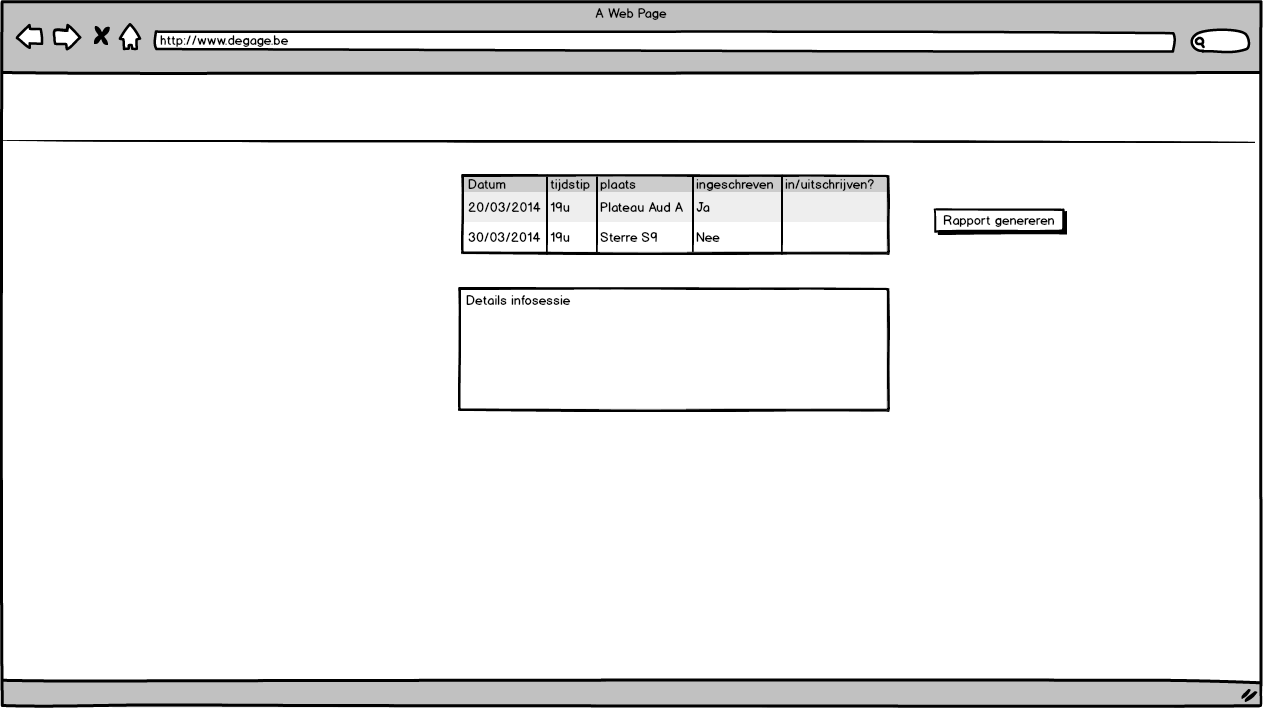
\includegraphics[width=\textwidth]{../../mockups/infosessies_autolener.png}\end{figure}

\begin{figure}[H]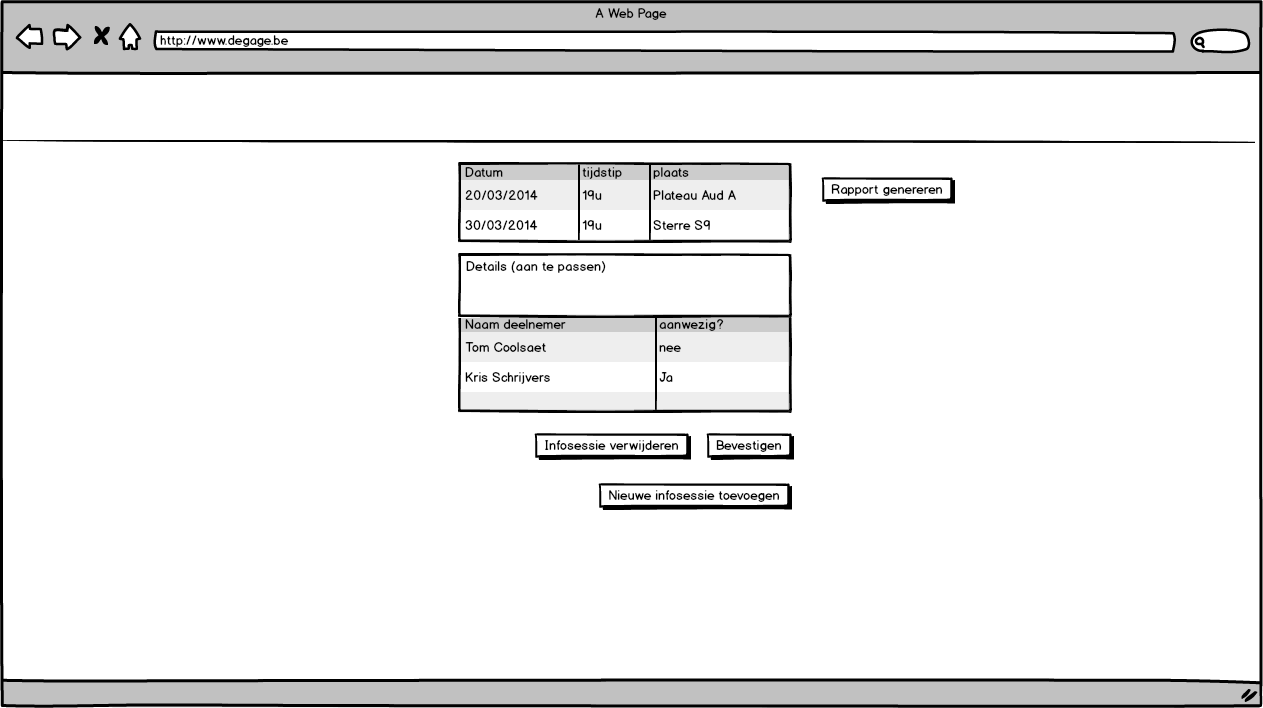
\includegraphics[width=\textwidth]{../../mockups/infosessies_beheerder.png}\end{figure}

\setcounter{section}{0}
\setcounter{subsection}{0}
\part{Editeerbare emails versturen door het systeem}

\section{Usecases}

\subsection{Een beheerder past een standaard-mail aan}
\begin{itemize}
\item \textbf{Precondities:} een beheerder met de machtiging om mails aan te passen en te versturen is ingelogd op het systeem.
\item \textbf{Trigger:} de beheerder selecteert om een bepaald standaard-mail aan te passen.
\item \textbf{Acties:} 
\begin{itemize}
	\item	Het systeem toont een editor aan de beheerder met hierin de huidige HTML-code (+ SCALA-code) van de mail.
	\item	De beheerder voert de gewenste wijzigingen uit.
	\item	Het systeem verifi\"{e}ert de correctheid van de nieuwe code.
		\begin{itemize}
			\item Indien de verificatie mislukt, worden de fouten afgeprint en moet de gebruiker de fouten eerst herstellen.
		\end{itemize}
\end{itemize}
\item \textbf{Postcondities:} Indien de verificatie lukt, is de code van de standaard-mail aangepast.
\end{itemize}

\subsection{Een beheerder stuurt een standaard-email naar een gebruiker}
\begin{itemize}
\item \textbf{Precondities:} een beheerder met de machtiging om mails aan te passen en te versturen is ingelogd op het systeem.
\item \textbf{Trigger:} de beheerder selecteert om een bepaald standaard-mail te versturen
\item \textbf{Acties:} 
\begin{itemize}
	\item	De beheerder selecteert een gebruiker of meerdere gebruikers (een volledige autogroep, alle gebruikers binnen een bepaalde regio, ...).
	\item	De beheerder selecteert \emph{versturen}.
\end{itemize}
\item \textbf{Postcondities:} Het systeem verstuurt een email naar de geselecteerde gebruikers.
\end{itemize}

\subsection{Het systeem verstuurt een notificatiemail naar een gebruiker}
\begin{itemize}
\item \textbf{Precondities:} /
\item \textbf{Trigger:} een event waarvoor een notificatiemail verstuurt moet worden doet zich voor (bijvoorbeeld: een gebruiker heeft 3 of meer openstaande ritten waarvan de ritgegevens ingevuld moeten worden).
\item \textbf{Acties:} 
\begin{itemize}
	\item	Het systeem verstuurt de notificatiemail horende bij het event.
\end{itemize}
\item \textbf{Postcondities:} De gebruiker ontvangt een notificatiemail.
\end{itemize}

\section{Mockups}

\begin{figure}[H]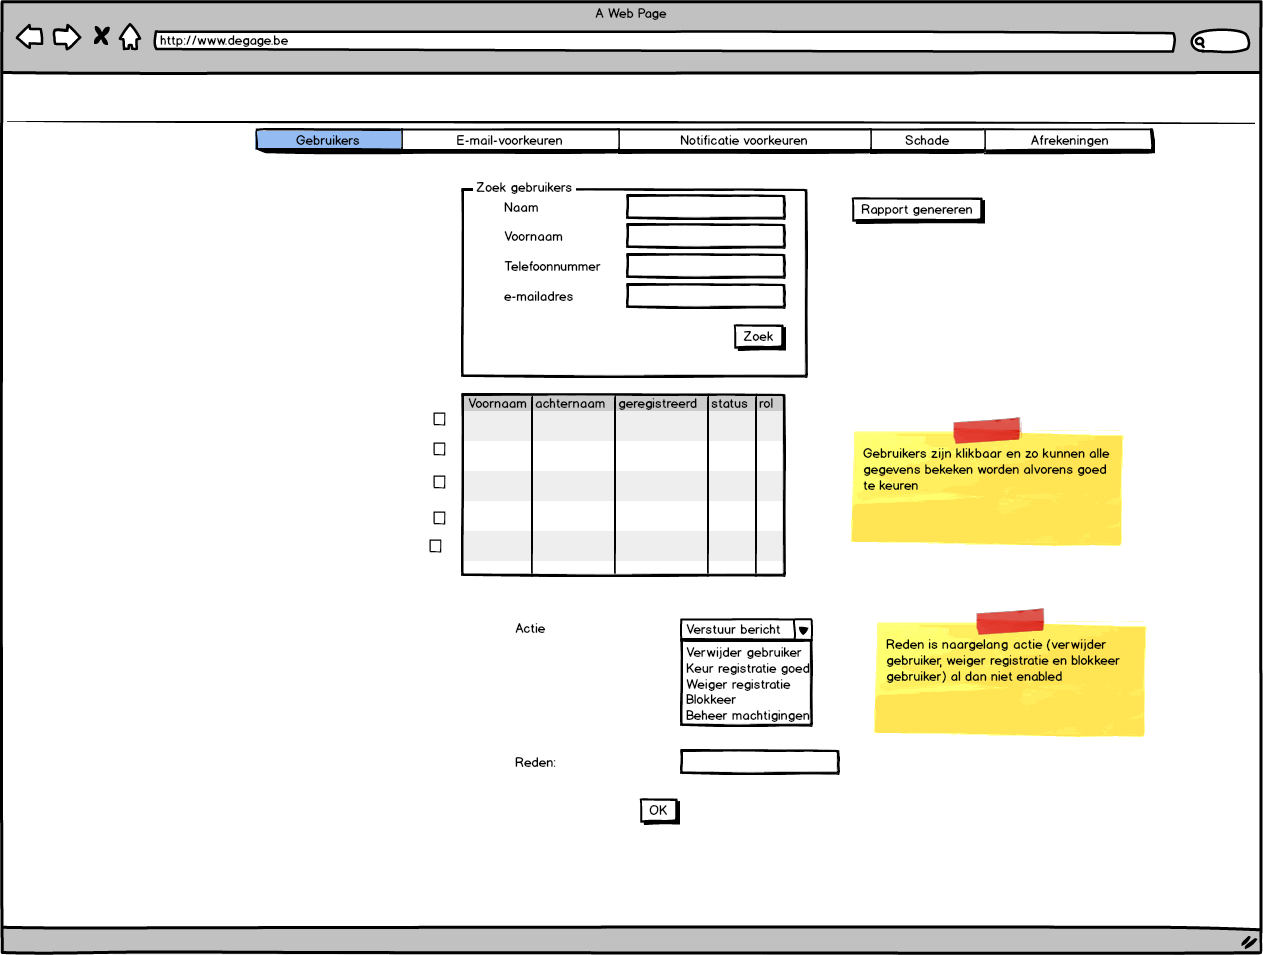
\includegraphics[width=\textwidth]{../../mockups/admin_dashboard_gebruikers.png}\end{figure}
\begin{figure}[H]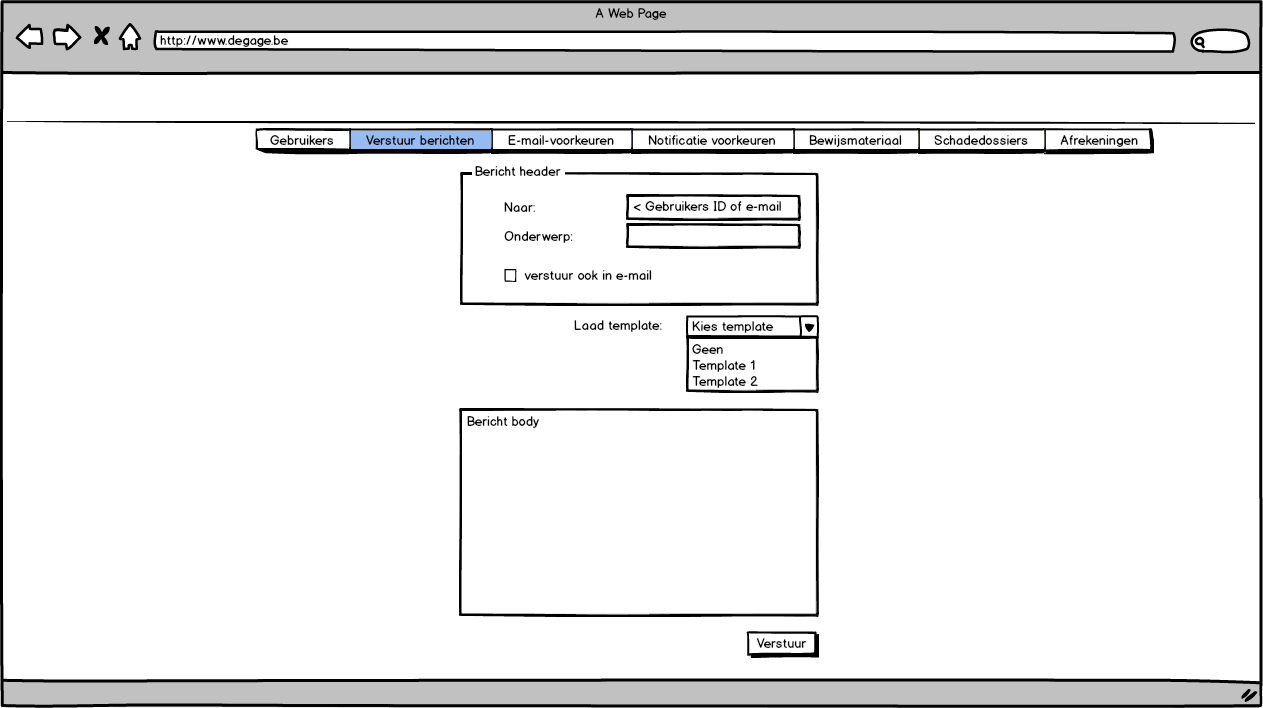
\includegraphics[width=\textwidth]{../../mockups/admin_dashboard_stuur_bericht.png}\end{figure}
\begin{figure}[H]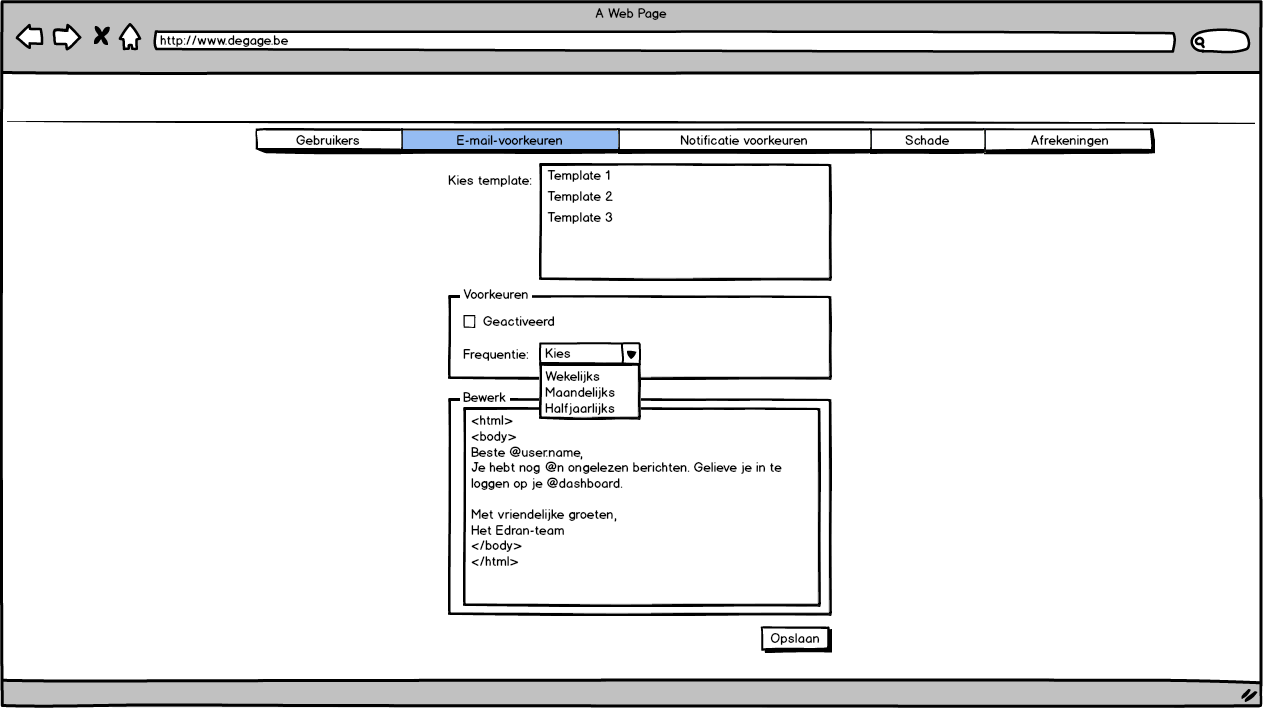
\includegraphics[width=\textwidth]{../../mockups/admin_dashboard_mailvoorkeuren.png}\end{figure}
\end{document}